\clearpage
\begin{flushright}
	\textit{Лекция №4}
	\textit{2015.09.15}
\end{flushright}

Процесс – единица декомпозиции, ему выделяются ресурсы. Он является владельцем ресурсов. 

\subsection{Виды ОС}
\begin{enumerate}
    \item однопрограммные пакетной обработки
    \item мультипрограммной пакетной обработки. (планирование на принципе распараллеливания функций. Программа выполняется до тех пор, пока не запросит доп. Ресурс системы или пока не придет более высокоприоритетный процесс, в случае поддержки вытеснения, может вытеснить)
    \item системы разделения времени, система квантования. (каждому выделяется квант процессорного времени. Процесс выполняется до тех пор, пока не истек квант, не начался процесс ввода/вывода или не вытеснен другим высокоприоритетным процессом.)
\end{enumerate}


\subsection{Алгоритмы планирования для систем пакетной обработки}
\begin{enumerate}
    \item FIFO. Не учитываются приоритеты, нет вытеснения.
    \item SJF. Короткие задания получают более высокий приоритет. Как результат – бесконечное откладывание. 
    \item HRN – наибольшее относительное время ответа. Приоритет вычисляется по формуле $P = (tw – ts) / ts$, где $ts$ – запрошенное время обслуживания. $tw$ – время ожидания.
    \item SRT наименьшее оставшееся время. Процесс может быть вытеснен, если в очередь готовых процессов поступит процесс, с меньшим оценочным временем откладывания. Тут процессы вытесняются.
\end{enumerate}

\subsection{Алгоритмы планирования для интерактивных систем}
\begin{enumerate}
    \item RR – процессы формируют очередь, но при истечении кванта они опять попадают в очередь. 
    \item Многоуровневые очереди. В системе процессы организуются в несколько очередей, наивысший приоритет имеет первая очередь. В неё попадают вновь созданные процессы и процессы, завершившие ожидание ввода вывода.  Если процесс не успел завершиться или попросить ввод/вывод, он поступает в следующей очередь. В конце – 4 очередь RR, в котором крутится холостой процесс.
    \item  адаптивное ?? планирование - учитывает объем занимаемое процессом физической памяти. Дополнительно оценивается объем памяти занимаемое процессом, а также учитывается, может ли процесс получить необходимое для дальнейшего выполнения объем физической памяти. Только в этом случае процесс получит квант процессорного времени. Если процесс не может получить объем физической памяти, то он может быть приостановлен до благоприятной ситуации.
\end{enumerate}

\begin{figure}[H]
  \centering
  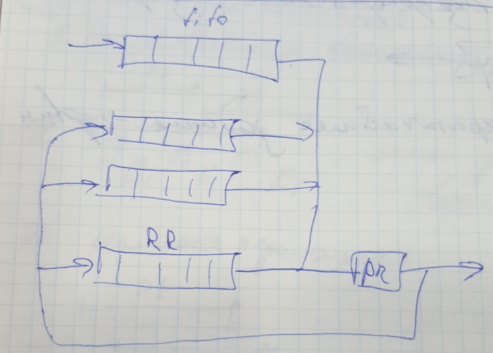
\includegraphics[width=\textwidth]{pic/1.png}
  \caption{Многоуровневые очереди}
\end{figure}

\section{Cоздание нового процесса}

fork() – создание нового процесса (порождение процесса). Процесс должен быть идентифицирован. В системе – одна главная таблица процесс. Поля – обычно указатели на другие структуры.  После этого может быть выделена память. Память в системе может быть выделена той частью системы, которая называется менеджер памяти. Он должен решить сколько и где выделить памяти. Если памяти недостаточно в данный момент, то процесс будет переведен в состояние «готов к запуску, выгружен», иначе «готов к запуску, в памяти».

Процесс часть времени выполняется в режиме пользователя и выполняет свой код, а часть времени – в режиме ядра и тогда выполняет реентерабельный код ОС. В процессе выполнения процесс запрашивает дополнительные ресурсы с помощью системных вызовов. Выполнив системный вызов процесс будет переведен в режим ядра. Системный вызов – программное прерывание. В режим ядра процесс будет возвращен, когда он обратиться к коду , который отсутствует в физической. В режиме ядра будет решено, блокировать процесс или ???.


\begin{figure}[H]
  \centering
  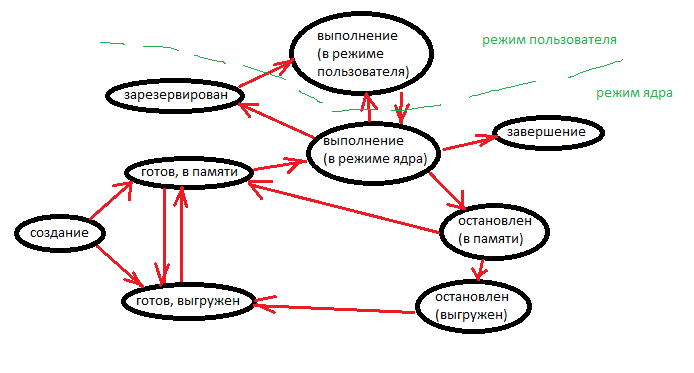
\includegraphics[width=\textwidth]{pic/2.png}
  \caption{pic}
\end{figure}

\subsection{Cобытия, переводящие систему в режим ядра (система прерывания)}
\begin{enumerate}
    \item Системные вызовы или программные прерывания. Выполняемая программа пользователя нуждается в ?? и выполняет системный вызов. АПИ – набор функций, которые предоставляет система. Ни одна система не позволяет процессам на прямую выполнять ввод/вывод, только через системный вызов.
    \item Исключения (устранимые, не устранимые). Системные вызовы и исключения – синхронные события по отношению к вашему процессу. Возникают в процессе выполнения программного кода. Исключения возникают в результате ошибок в программе (не устранимым, например - деление на ноль). Устранимое – страничное прерывание, необходимая страница будет загружена в память и программа продолжит выполнение.
    \item Аппаратные прерывания. Сугубо асинхронные события в системе. Также имеют различный характер в системе. Самое массовое – прерывания от внешних устройств. Второй тип – прерывание от системного таймера, которое выполняется по тику(выделенный импульс) 18,3 раз в секунду.  Третий тип – прерывание от действий оператора (ctrl alt del , ctrl + C = завершение процесса в unix)
\end{enumerate}

Когда выполняется запрос на ввод вывод, в режиме ядра вызывается драйвер, он формирует запрос, который посылается ???. По завершении операции ввода/вывода контроллер посылает сигнал прерывания в контроллер прерывания и он формирует сигнал прерывания для процессора.

\chapter{Потоки}
Сохранение аппаратного контекста выполняется аппаратно (pusha). Процесс обладает выделенными ему ресурсами, которые описываются таблицами.  При переходе к другому процессу происходит переключение полного контекста. Это долго, поэтому появилась идея потоков. 

\paragraph{Виды потоков}: 
\begin{enumerate}
    \item Потоки ядра;
    \item Легковесные процессы;
    \item Пользовательские нити. (выполняются библиотеками).
\end{enumerate}

Поток – непрерывная часть кода, выполняющаяся параллельно с другими потоками кода. Поток не имеет собственного адресного пространства. Владельцем ресурсов является процесс. Поток владеет аппаратным контекстом и счетчиком команд. 

\begin{figure}[H]
  \centering
  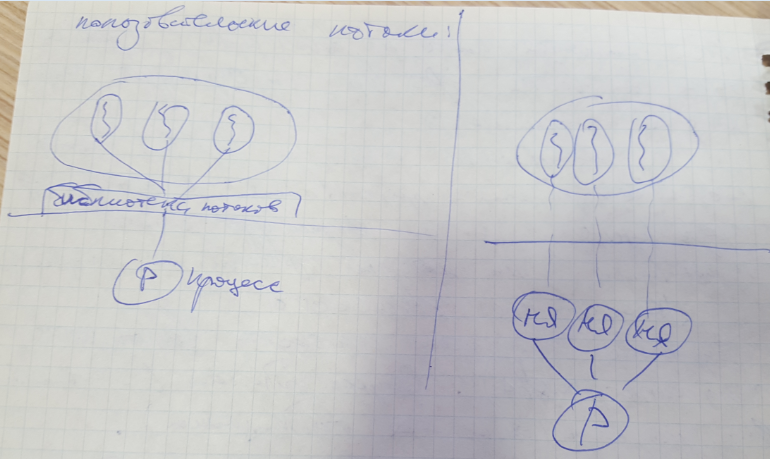
\includegraphics[width=\textwidth]{pic/3.png}
  \caption{Виды потоков}
\end{figure}
